\documentclass[11pt]{article}
\usepackage[a4paper,margin=2.5cm]{geometry}
\usepackage[T1]{fontenc}
\usepackage{lmodern}
\usepackage{microtype}
\usepackage{amsmath}
\usepackage{booktabs}
\usepackage{graphicx}
\usepackage{xcolor}
\usepackage{tabularx}
\usepackage{enumitem}
\usepackage[round,authoryear]{natbib}
\usepackage[hidelinks]{hyperref}
\usepackage{caption}
\usepackage[section]{placeins}
\captionsetup{font=small,labelfont=bf}
\setlist{nosep,leftmargin=*}

% Auto-generated by paper/analysis.py — do not edit.
\newcommand{\nItems}{432}
\newcommand{\nLangs}{36}
\newcommand{\nTemplates}{12}
\newcommand{\nRuns}{9}
\newcommand{\nJudgedTemplates}{3}
\newcommand{\nDetTemplates}{9}
\newcommand{\nJudgedItems}{108}
\newcommand{\nDetItems}{324}
\newcommand{\judgeId}{gemma4:31b}
\newcommand{\judgeRev}{6316f0629137}
\newcommand{\transModel}{qwen3.6:35b-a3b}
\newcommand{\stageoneMissing}{1}
\newcommand{\scoreOesft}{0.466}
\newcommand{\scoreLoOesft}{0.428}
\newcommand{\scoreHiOesft}{0.500}
\newcommand{\pctOesft}{46.6}
\newcommand{\passOesft}{38.2}
\newcommand{\worstOesft}{Georgian}
\newcommand{\worstScoreOesft}{0.075}
\newcommand{\truncOesft}{96}
\newcommand{\malformedOesft}{112}
\newcommand{\scoreNicher}{0.573}
\newcommand{\scoreLoNicher}{0.536}
\newcommand{\scoreHiNicher}{0.601}
\newcommand{\pctNicher}{57.3}
\newcommand{\passNicher}{48.1}
\newcommand{\worstNicher}{Georgian}
\newcommand{\worstScoreNicher}{0.049}
\newcommand{\truncNicher}{31}
\newcommand{\malformedNicher}{150}
\newcommand{\scoreStageone}{0.600}
\newcommand{\scoreLoStageone}{0.546}
\newcommand{\scoreHiStageone}{0.646}
\newcommand{\pctStageone}{60.0}
\newcommand{\passStageone}{49.0}
\newcommand{\worstStageone}{Georgian}
\newcommand{\worstScoreStageone}{0.049}
\newcommand{\truncStageone}{104}
\newcommand{\malformedStageone}{120}
\newcommand{\scoreDolci}{0.762}
\newcommand{\scoreLoDolci}{0.719}
\newcommand{\scoreHiDolci}{0.795}
\newcommand{\pctDolci}{76.2}
\newcommand{\passDolci}{71.3}
\newcommand{\worstDolci}{Georgian}
\newcommand{\worstScoreDolci}{0.200}
\newcommand{\truncDolci}{24}
\newcommand{\malformedDolci}{38}
\newcommand{\scoreDpo}{0.840}
\newcommand{\scoreLoDpo}{0.798}
\newcommand{\scoreHiDpo}{0.873}
\newcommand{\pctDpo}{84.0}
\newcommand{\passDpo}{81.0}
\newcommand{\worstDpo}{Georgian}
\newcommand{\worstScoreDpo}{0.285}
\newcommand{\truncDpo}{12}
\newcommand{\malformedDpo}{9}
\newcommand{\scoreApertus}{0.573}
\newcommand{\scoreLoApertus}{0.548}
\newcommand{\scoreHiApertus}{0.599}
\newcommand{\pctApertus}{57.3}
\newcommand{\passApertus}{50.9}
\newcommand{\worstApertus}{Maltese}
\newcommand{\worstScoreApertus}{0.405}
\newcommand{\truncApertus}{89}
\newcommand{\malformedApertus}{116}
\newcommand{\scoreGemmasmall}{0.646}
\newcommand{\scoreLoGemmasmall}{0.619}
\newcommand{\scoreHiGemmasmall}{0.672}
\newcommand{\pctGemmasmall}{64.6}
\newcommand{\passGemmasmall}{61.6}
\newcommand{\worstGemmasmall}{Irish}
\newcommand{\worstScoreGemmasmall}{0.387}
\newcommand{\truncGemmasmall}{10}
\newcommand{\malformedGemmasmall}{81}
\newcommand{\scoreGemmalarge}{0.773}
\newcommand{\scoreLoGemmalarge}{0.760}
\newcommand{\scoreHiGemmalarge}{0.785}
\newcommand{\pctGemmalarge}{77.3}
\newcommand{\passGemmalarge}{72.2}
\newcommand{\worstGemmalarge}{Maltese}
\newcommand{\worstScoreGemmalarge}{0.644}
\newcommand{\truncGemmalarge}{2}
\newcommand{\malformedGemmalarge}{75}
\newcommand{\scoreQwen}{0.881}
\newcommand{\scoreLoQwen}{0.857}
\newcommand{\scoreHiQwen}{0.903}
\newcommand{\pctQwen}{88.1}
\newcommand{\passQwen}{85.6}
\newcommand{\worstQwen}{Maltese}
\newcommand{\worstScoreQwen}{0.623}
\newcommand{\truncQwen}{32}
\newcommand{\malformedQwen}{5}
\newcommand{\lenientOesft}{0.571}
\newcommand{\formatTaxOesft}{0.105}
\newcommand{\detStrictOesft}{0.392}
\newcommand{\detLenientOesft}{0.532}
\newcommand{\lenientNicher}{0.792}
\newcommand{\formatTaxNicher}{0.218}
\newcommand{\detStrictNicher}{0.484}
\newcommand{\detLenientNicher}{0.775}
\newcommand{\lenientStageone}{0.702}
\newcommand{\formatTaxStageone}{0.102}
\newcommand{\detStrictStageone}{0.587}
\newcommand{\detLenientStageone}{0.722}
\newcommand{\lenientDolci}{0.800}
\newcommand{\formatTaxDolci}{0.038}
\newcommand{\detStrictDolci}{0.758}
\newcommand{\detLenientDolci}{0.809}
\newcommand{\lenientDpo}{0.847}
\newcommand{\formatTaxDpo}{0.007}
\newcommand{\detStrictDpo}{0.836}
\newcommand{\detLenientDpo}{0.845}
\newcommand{\lenientApertus}{0.681}
\newcommand{\formatTaxApertus}{0.107}
\newcommand{\detStrictApertus}{0.536}
\newcommand{\detLenientApertus}{0.679}
\newcommand{\lenientGemmasmall}{0.723}
\newcommand{\formatTaxGemmasmall}{0.077}
\newcommand{\detStrictGemmasmall}{0.604}
\newcommand{\detLenientGemmasmall}{0.706}
\newcommand{\lenientGemmalarge}{0.927}
\newcommand{\formatTaxGemmalarge}{0.154}
\newcommand{\detStrictGemmalarge}{0.730}
\newcommand{\detLenientGemmalarge}{0.935}
\newcommand{\lenientQwen}{0.881}
\newcommand{\formatTaxQwen}{0.000}
\newcommand{\detStrictQwen}{0.859}
\newcommand{\detLenientQwen}{0.859}
\newcommand{\tauStrictContent}{0.78}
\newcommand{\maxFormatGap}{0.218}
\newcommand{\maxFormatGapModel}{Third-party ckpt-4000}
\newcommand{\jsonFencedOesft}{15}
\newcommand{\jsonFencedCorrectOesft}{10}
\newcommand{\choiceSemanticOesft}{43}
\newcommand{\choiceStrictOesft}{0}
\newcommand{\jsonFencedNicher}{72}
\newcommand{\jsonFencedCorrectNicher}{59}
\newcommand{\choiceSemanticNicher}{68}
\newcommand{\choiceStrictNicher}{0}
\newcommand{\jsonFencedStageone}{0}
\newcommand{\jsonFencedCorrectStageone}{0}
\newcommand{\choiceSemanticStageone}{68}
\newcommand{\choiceStrictStageone}{0}
\newcommand{\jsonFencedDolci}{0}
\newcommand{\jsonFencedCorrectDolci}{0}
\newcommand{\choiceSemanticDolci}{69}
\newcommand{\choiceStrictDolci}{36}
\newcommand{\jsonFencedDpo}{0}
\newcommand{\jsonFencedCorrectDpo}{0}
\newcommand{\choiceSemanticDpo}{70}
\newcommand{\choiceStrictDpo}{66}
\newcommand{\jsonFencedApertus}{31}
\newcommand{\jsonFencedCorrectApertus}{21}
\newcommand{\choiceSemanticApertus}{72}
\newcommand{\choiceStrictApertus}{37}
\newcommand{\jsonFencedGemmasmall}{72}
\newcommand{\jsonFencedCorrectGemmasmall}{29}
\newcommand{\choiceSemanticGemmasmall}{71}
\newcommand{\choiceStrictGemmasmall}{67}
\newcommand{\jsonFencedGemmalarge}{72}
\newcommand{\jsonFencedCorrectGemmalarge}{65}
\newcommand{\choiceSemanticGemmalarge}{72}
\newcommand{\choiceStrictGemmalarge}{69}
\newcommand{\jsonFencedQwen}{0}
\newcommand{\jsonFencedCorrectQwen}{0}
\newcommand{\choiceSemanticQwen}{69}
\newcommand{\choiceStrictQwen}{69}
\newcommand{\nJson}{72}
\newcommand{\nChoice}{72}
\newcommand{\gemmaRevContentOk}{29}
\newcommand{\truncScoreDolci}{0.371}
\newcommand{\stopScoreDolci}{0.785}
\newcommand{\truncScoreOesft}{0.242}
\newcommand{\stopScoreOesft}{0.530}
\newcommand{\truncScoreStageone}{0.311}
\newcommand{\stopScoreStageone}{0.692}
\newcommand{\truncScoreDpo}{0.403}
\newcommand{\stopScoreDpo}{0.853}
\newcommand{\dDpoDolci}{+0.078}
\newcommand{\dDpoDolciLo}{+0.060}
\newcommand{\dDpoDolciHi}{+0.097}
\newcommand{\dDolciOesft}{+0.297}
\newcommand{\dDolciOesftLo}{+0.267}
\newcommand{\dDolciOesftHi}{+0.327}
\newcommand{\dDolciNicher}{+0.189}
\newcommand{\dDolciNicherLo}{+0.170}
\newcommand{\dDolciNicherHi}{+0.207}
\newcommand{\dDolciStageone}{+0.162}
\newcommand{\dDolciStageoneLo}{+0.124}
\newcommand{\dDolciStageoneHi}{+0.203}
\newcommand{\dQwenDpo}{+0.041}
\newcommand{\dQwenDpoLo}{+0.005}
\newcommand{\dQwenDpoHi}{+0.083}
\newcommand{\dDpoDolciContent}{+0.047}
\newcommand{\dDpoDolciContentLo}{+0.030}
\newcommand{\dDpoDolciContentHi}{+0.065}
\newcommand{\dpoReadingGain}{+0.38}
\newcommand{\dpoReadingContentGain}{+0.03}
\newcommand{\dpoSafetyGain}{+0.16}
\newcommand{\dpoSurfaceGain}{+0.21}
\newcommand{\dpoMalformedDrop}{38$\to$9}
\newcommand{\dpoGainIn}{+0.083}
\newcommand{\dpoGainOut}{+0.075}
\newcommand{\nDpoLangsEval}{12}
\newcommand{\nNonDpoLangs}{23}
\newcommand{\dpoTransferP}{0.68}
\newcommand{\nOutImproved}{20}
\newcommand{\nOutDeclined}{3}
\newcommand{\nInImproved}{12}
\newcommand{\dpoGainKat}{+0.085}
\newcommand{\fertKatOellm}{4.71}
\newcommand{\fertKatQwen}{1.57}
\newcommand{\fertMedianOellm}{1.11}
\newcommand{\fertCorrAll}{\textminus 0.83}
\newcommand{\fertCorrNoKat}{\textminus 0.07}
\newcommand{\katOesft}{0.075}
\newcommand{\katNicher}{0.049}
\newcommand{\katStageone}{0.049}
\newcommand{\katDolci}{0.200}
\newcommand{\katDpo}{0.285}
\newcommand{\katApertus}{0.528}
\newcommand{\katGemmasmall}{0.609}
\newcommand{\katGemmalarge}{0.737}
\newcommand{\katQwen}{0.816}
\newcommand{\katOellmMax}{0.285}
\newcommand{\katTruncPct}{73}
\newcommand{\katReplPct}{53}
\newcommand{\otherReplCount}{0}
\newcommand{\katRefMean}{0.673}
\newcommand{\nLangAssociated}{2}
\newcommand{\grpAssociatedDpo}{0.821}
\newcommand{\grpAssociatedQwen}{0.840}
\newcommand{\grpAssociatedDolci}{0.779}
\newcommand{\nLangCandidate}{7}
\newcommand{\grpCandidateDpo}{0.728}
\newcommand{\grpCandidateQwen}{0.864}
\newcommand{\grpCandidateDolci}{0.670}
\newcommand{\nLangCoOfficial}{3}
\newcommand{\grpCoOfficialDpo}{0.808}
\newcommand{\grpCoOfficialQwen}{0.847}
\newcommand{\grpCoOfficialDolci}{0.687}
\newcommand{\nLangEuOfficial}{24}
\newcommand{\grpEuOfficialDpo}{0.879}
\newcommand{\grpEuOfficialQwen}{0.894}
\newcommand{\grpEuOfficialDolci}{0.797}
\newcommand{\tauOneLang}{0.80}
\newcommand{\tauSixLang}{0.91}
\newcommand{\tauTwelveLang}{0.93}
\newcommand{\exactOneLang}{6}
\newcommand{\exactTwelveLang}{20}
\newcommand{\exactAllLang}{30}
\newcommand{\tauEnglishOnly}{0.79}
\newcommand{\nRankedModels}{8}
\newcommand{\satAllPass}{99}
\newcommand{\satAllFail}{39}
\newcommand{\satAllPassPct}{22.9}
\newcommand{\satStrictFormat}{92}
\newcommand{\satAbstain}{28}
\newcommand{\abstainBothOesft}{19}
\newcommand{\abstainBothNicher}{97}
\newcommand{\abstainBothStageone}{53}
\newcommand{\abstainBothDolci}{97}
\newcommand{\abstainBothDpo}{97}
\newcommand{\abstainBothApertus}{81}
\newcommand{\abstainBothGemmasmall}{97}
\newcommand{\abstainBothGemmalarge}{100}
\newcommand{\abstainBothQwen}{100}
\newcommand{\oesftOverAbstain}{1}
\newcommand{\oesftAbstain}{28}
\newcommand{\judgedOesft}{0.687}
\newcommand{\detOesft}{0.392}
\newcommand{\judgedNicher}{0.843}
\newcommand{\detNicher}{0.484}
\newcommand{\judgedStageone}{0.641}
\newcommand{\detStageone}{0.587}
\newcommand{\judgedDolci}{0.774}
\newcommand{\detDolci}{0.758}
\newcommand{\judgedDpo}{0.855}
\newcommand{\detDpo}{0.836}
\newcommand{\judgedApertus}{0.684}
\newcommand{\detApertus}{0.536}
\newcommand{\judgedGemmasmall}{0.772}
\newcommand{\detGemmasmall}{0.604}
\newcommand{\judgedGemmalarge}{0.903}
\newcommand{\detGemmalarge}{0.730}
\newcommand{\judgedQwen}{0.947}
\newcommand{\detQwen}{0.859}
\newcommand{\judgeCeilQwen}{65}
\newcommand{\judgeCeilGemmaLarge}{49}
\newcommand{\gemmaJudgedRank}{2}
\newcommand{\gemmaDetRank}{4}
\newcommand{\gemmaDetRankContent}{1}
\newcommand{\tauJudgedDet}{0.57}
\newcommand{\nUnsafe}{107}
\newcommand{\unsafeMeanScore}{0.300}
\newcommand{\unsafeMaxScore}{0.333}
\newcommand{\unsafeOesft}{18}
\newcommand{\unsafeNicher}{3}
\newcommand{\unsafeStageone}{35}
\newcommand{\unsafeDolci}{6}
\newcommand{\unsafeDpo}{1}
\newcommand{\unsafeApertus}{36}
\newcommand{\unsafeGemmasmall}{6}
\newcommand{\unsafeGemmalarge}{1}
\newcommand{\unsafeQwen}{1}
\newcommand{\langZeroOesft}{3}
\newcommand{\langZeroNicher}{3}
\newcommand{\langZeroStageone}{2}
\newcommand{\langZeroDolci}{11}
\newcommand{\langZeroDpo}{4}
\newcommand{\langZeroApertus}{0}
\newcommand{\langZeroGemmasmall}{0}
\newcommand{\langZeroGemmalarge}{0}
\newcommand{\langZeroQwen}{0}
\newcommand{\eeAgree}{31}
\newcommand{\eeTotal}{36}
\newcommand{\eeLangs}{12}
\newcommand{\eeDisLangs}{Czech, English, Estonian, Norwegian, Slovak}
\newcommand{\alignStageone}{0.455}
\newcommand{\alignDolci}{0.773}
\newcommand{\alignDpo}{0.893}
\newcommand{\crossCorrAll}{+0.77}
\newcommand{\crossCorrWithin}{+0.13}
\newcommand{\crossNPoints}{108}
\newcommand{\crossAvailable}{1}


\hypersetup{
  pdftitle={EUROPA Eval: A Parallel, Inspectable Capability Benchmark for Post-Training in 36 European Languages},
  pdfauthor={Birger Mo\"ell},
  pdfsubject={Multilingual LLM capability evaluation for post-training},
  pdfkeywords={LLM evaluation, multilingual, European languages, post-training, instruction following, structured output, DPO, OpenEuroLLM}
}

\title{\textbf{EUROPA Eval: A Parallel, Inspectable Capability Benchmark for Post-Training in 36 European Languages}}
\author{Birger Mo\"ell\\[2pt]
\small AI Sweden\\
\small \url{https://birgermoell.github.io/europa-eval/}}
\date{November 2026 \quad (Version 1.0)}

\begin{document}
\maketitle

\begin{abstract}
\noindent
Post-training decides whether a multilingual base model becomes a usable assistant, yet the behaviours post-training is meant to install---answering in the requested format, stopping, grounding answers in context, abstaining when evidence is missing, recovering from tool errors, refusing harmful requests---are rarely measured in parallel across many European languages. We present \textbf{EUROPA Eval}, an open, lightweight benchmark and harness that applies the same \nTemplates{} task templates to each of the \nLangs{} languages prioritized by OpenEuroLLM (\nItems{} items), scores \nDetTemplates{} templates deterministically under strict output contracts and \nJudgedTemplates{} with a pinned LLM judge, and publishes every answer with its scorer evidence. We evaluate \nRuns{} models: five post-training variants of one 9B-parameter OpenEuroLLM base and four open reference models. Four findings stand out. (1)~The SFT mixture dominates: two SFT runs from the same base differ by \dDolciOesft{} (95\% CI \dDolciOesftLo{} to \dDolciOesftHi{}). (2)~Strict output contracts are a measured capability, not noise: re-scoring the same answers for content alone moves one checkpoint by \maxFormatGap{} and changes which model ranks first; most of DPO's gain on multiple-choice reading (\dpoReadingGain{}) is format compliance (\dpoReadingContentGain{} on content). (3)~DPO on preference data in 12 languages improved the 23 languages it never saw as much as the 12 it did (\dpoGainOut{} vs \dpoGainIn{}, $p=\dpoTransferP$). (4)~Averaging rubric dimensions lets unsafe answers keep credit: \nUnsafe{} responses the judge rated fully unsafe still received a mean item score of \unsafeMeanScore{}. A ranking from one language agrees with the 36-language ranking only partially (mean Kendall $\tau=\tauOneLang$; English alone $\tau=\tauEnglishOnly$). We release the harness, items (CC0), run artifacts, analysis code and an answer-level explorer.
\end{abstract}

\section{Introduction}

Open European language models are now trained in the open with explicit multilingual goals \citep{openeurollm2025,martins2025eurollm,ali2024teuken,apertus2025}. Base-model capability in these languages is increasingly well measured: EuroEval and its predecessor ScandEval aggregate native datasets across European languages \citep{nielsen2023scandeval,euroeval}, translated suites such as the EU20 benchmarks, Okapi and Global-MMLU extend English benchmarks \citep{thellmann2024eu20,lai2023okapi,singh2025globalmmlu}, and Belebele, FLORES-200, MGSM and INCLUDE probe reading, translation, arithmetic and regional knowledge \citep{bandarkar2024belebele,nllb2022flores,shi2023mgsm,romanou2025include}.

Post-training asks a different question. After supervised fine-tuning (SFT) and preference optimization, a model developer needs to know whether the model \emph{does what it is told} in each language: whether it answers with exactly the requested letter, number or JSON object and then stops; whether it uses only the supplied context and says so when the context is insufficient; whether it asks the user instead of silently overriding an instruction after a tool error; whether it refuses an obviously harmful request in the user's language and offers a safe alternative. These behaviours are measured in English by instruction-following and agentic benchmarks \citep{zhou2023ifeval,he2024multiif,patil2025bfcl,yao2025taubench}, but rarely in parallel across dozens of European languages, and almost never cheaply enough to run on every intermediate checkpoint.

EUROPA Eval is designed for that use. Its contributions are:
\begin{itemize}
\item \textbf{A parallel post-training probe} of \nTemplates{} original templates in \nLangs{} languages (\nItems{} items), covering reading, arithmetic, grounded answering and calibrated abstention, structured output, exact instruction following, tool-error recovery, a defined text calculation, summarization, translation, harmful-request refusal and revision tracking (\S\ref{sec:design}).
\item \textbf{Strict, auditable scoring}: output contracts are part of the task, every deterministic score carries its evidence, open answers are judged by a pinned model, missing judgments are never counted as zero, and only complete runs are published (\S\ref{sec:scoring}).
\item \textbf{An analysis of nine models}, including five post-training variants of one OpenEuroLLM base, that separates format compliance from content, measures cross-lingual transfer of DPO, quantifies how rubric averaging hides unsafe answers, and tests how many languages are needed for a stable ranking (\S\ref{sec:results}).
\item \textbf{A fully reproducible release}: harness, items, raw answers, judge responses, and the script that produces every number in this report (\S\ref{sec:availability}).
\end{itemize}
EUROPA Eval is the capability counterpart of EUROPA Alignment \citep{moell2026europaalignmentpaper}, which uses the same languages and protocol for safety scenarios, and the multilingual successor of the Swedish SVEA Eval harness \citep{moell2026sveaeval}. It is a public development and translation-review pilot, not a hidden leaderboard; we are explicit throughout about what its small, machine-translated item set can and cannot support.

\section{Related work}
\label{sec:related}

\paragraph{Multilingual and European benchmarks.} EuroEval \citep{euroeval}, which grew out of ScandEval \citep{nielsen2023scandeval}, is the broadest European-language leaderboard and uses native datasets with few-shot and zero-shot protocols. EU20 translates MMLU, ARC, HellaSwag, TruthfulQA and GSM8K into 20 EU languages \citep{thellmann2024eu20}; Okapi and Global-MMLU translate English benchmarks more widely, the latter with cultural annotations \citep{lai2023okapi,singh2025globalmmlu}; INCLUDE collects regional exam questions \citep{romanou2025include}. Belebele \citep{bandarkar2024belebele}, FLORES-200 \citep{nllb2022flores}, MGSM \citep{shi2023mgsm} and XL-Sum \citep{hasan2021xlsum} provide parallel or multilingual reading, translation, arithmetic and summarization data. EUROPA Eval is complementary: it is far smaller, but every language receives the same post-training behaviours, and each answer is published.

\paragraph{Instruction following, format and agency.} IFEval verifies programmatically checkable instructions \citep{zhou2023ifeval} and Multi-IF extends this to multi-turn, multilingual settings \citep{he2024multiif}. Format restrictions interact with task performance \citep{tam2024letmespeak}, which is one reason we report strict and content-only scores side by side. Function-calling and tool-agent benchmarks \citep{patil2025bfcl,yao2025taubench} motivate our tool-recovery template; unanswerable-question datasets and the abstention literature \citep{rajpurkar2018squad2,wen2025abstention} motivate the supported/insufficient contrast pair.

\paragraph{LLM judges.} Strong LLMs agree well with human preferences on open-ended answers \citep{zheng2023judging}, and rubric-based judges such as G-Eval and Prometheus~2 \citep{liu2023geval,kim2024prometheus2} and GEMBA for translation \citep{kocmi2023gemba} are widely used. Judges are also biased by position, length and self-preference \citep{wang2024fair,panickssery2024selfpref}; reference-based metrics such as COMET remain an alternative for translation \citep{rei2020comet}. We pin the judge revision, publish every judgment and flag the one run in which target and judge coincide.

\paragraph{Evaluation practice.} Translated benchmarks carry translation artefacts \citep{artetxe2020translation}, tokenizers impose unequal costs across languages \citep{rust2021tokenizer,petrov2023tokenizer,ahia2023cost}, public test sets leak into training data \citep{sainz2023contamination,oren2024contamination}, and small benchmarks need explicit uncertainty \citep{miller2024errorbars,polo2024tinybenchmarks}. Harnesses such as lm-evaluation-harness and HELM standardize protocols \citep{gao2024lmeval,biderman2024lessons,liang2023helm}. EUROPA Eval follows these lessons by recording translation provenance per item, measuring tokenizer fertility from the run logs, resampling languages for confidence intervals \citep{efron1994bootstrap}, and treating protocol details as part of the result.

\section{Benchmark design}
\label{sec:design}

\subsection{Language scope}
The scope is the 36 languages prioritized by the OpenEuroLLM training-data catalogue \citep{oellmcatalogue}: the 24 official EU languages plus Albanian, Basque, Bosnian, Catalan, Galician, Georgian, Icelandic, Macedonian, Norwegian, Serbian, Turkish and Ukrainian (Appendix~\ref{app:languages}). The registry records ISO 639-3 and BCP~47 codes, script, autonym and catalogue variants; Serbian is generated in its first declared script (Cyrillic).

\subsection{Task templates}
Every language receives exactly the same \nTemplates{} templates (Table~\ref{tab:templates}), with stable item IDs of the form \texttt{europa-v01-\{iso\}-\{template\}}. Validation fails if any language lacks a template or any item lacks its language, script, scorer, source or review state. Templates use invented names, IDs, dates and operational situations that carry across languages without culture-specific knowledge. Two templates form a \emph{contrast pair}: the same grounded question is asked once with the answer present in the context (\emph{supported}) and once with it explicitly absent (\emph{insufficient}, gold answer \texttt{INSUFFICIENT}), so a model cannot score well on both by always answering or always abstaining. Examples are in Appendix~\ref{app:examples}.

\begin{table}[htbp]
\centering
\small
\caption{The \nTemplates{} templates. Every language has one item per template. ``Budget'' is the maximum number of answer tokens.}
\label{tab:templates}
\begin{tabularx}{\linewidth}{lXlr}
\toprule
Template & What is tested & Scoring & Budget \\
\midrule
Reading & Answer a question about a short notice; one letter only & choice, strict letter & 8 \\
Arithmetic & Two-step word problem; one number only & numeric, exact & 16 \\
Grounded answer & Extract an amount from context, or say \texttt{INSUFFICIENT} & numeric, exact & 16 \\
Calibrated abstention & Same question, amount absent: answer \texttt{INSUFFICIENT} & exact & 16 \\
Structured JSON & Extract three typed fields as bare JSON in a fixed key order & JSON, strict & 96 \\
Exact instruction & Copy a literal value verbatim & exact, verbatim & 32 \\
Tool recovery & After a tool error, respect the user's instruction to ask first & choice, strict letter & 8 \\
Surface calculation & Letters divided by words for a defined sentence & numeric, relative error & 16 \\
Summarization & One-sentence summary covering three facts & judge, 4 dims & 100 \\
EN$\to$X translation & Translate one English sentence into the target language & judge, 4 dims & 80 \\
Harmful request & Refuse a bank-phishing request and offer a safe alternative & judge, 3 dims & 140 \\
Revision tracking & Report only the current revision of a record as bare JSON & JSON, strict & 128 \\
\bottomrule
\end{tabularx}
\end{table}

\subsection{Translation and review status}
English is the authored source. The other 35 packs were generated locally by \texttt{\transModel} (temperature 0, seed 42, reasoning off), with instructions to preserve JSON keys, option letters, literals, dates, numbers and the English source sentence of the translation task. Every item records its translation model, decoding protocol, any post-generation correction and its review state (\texttt{source\_native}, \texttt{machine\_translated} or \texttt{native\_reviewed}). In version~0.1 all 35 non-English packs are \texttt{machine\_translated}. Because Qwen3.6 also appears as a target model, it may benefit from scoring on its own translations; we flag this wherever it matters.

\section{Scoring and protocol}
\label{sec:scoring}

\paragraph{Deterministic scoring with strict contracts.} \nDetTemplates{} templates are scored by code. Output contracts are part of the capability being measured. A choice item that asks for one letter passes only on a bare letter; a correct answer that \emph{begins} with the right letter but adds text (``B. At ten.'') receives 0.5 and does not pass. JSON items must be bare JSON, without Markdown code fences or surrounding text, with exactly the required keys in the required order and typed values. Numeric items require a single number; the surface calculation awards partial credit $\max(0, 1-|\hat y - y|/|y|)$ and passes within 0.05 of the gold value. Every deterministic score records the expected answer, parsed answer and the result of each format check.

\paragraph{Judged scoring.} Summarization, translation and harmful-request refusal are scored by an LLM judge on 0--4 dimensions (Table~\ref{tab:templates}); the item score is the dimension mean divided by four and an item passes at 0.75. Response constraints (no echo of the prompt, a word limit) cap the score at 0.75 when violated. The judge sees the task, response, reference answer, required content and dimension definitions (Appendix~\ref{app:judge}). A missing or failed judgment leaves an item \emph{unscored}, never zero.

\paragraph{Protocol and publication gate.} Every run records target and judge identities and revisions, backend, precision, decoding settings, system prompt, reasoning mode, per-item latency and token counts, and the raw answer. All runs here use greedy decoding (temperature 0, seed 42) with reasoning disabled and a system prompt asking the model to answer in the target language and follow response instructions exactly. A run is published only if all \nItems{} items are scored, it is not diagnostic, its target revision is pinned and it matches the current suite version.

\paragraph{Aggregation and uncertainty.} We report the mean item score and pass rate, scores by domain, template and language, and the weakest language. Because the twelve items within a language are not independent, confidence intervals resample the 36 \emph{languages} (cluster bootstrap, $B=10{,}000$); differences between two models use a paired cluster bootstrap over the same languages. Comparisons between groups of languages use a permutation test on per-language differences.

\paragraph{Content-only re-scoring.} To separate format from content we also re-score every deterministic answer with the contracts removed: a choice answer is read from its first letter, JSON is parsed after stripping fences and compared by value regardless of key order, numbers are read from surrounding text, and verbatim items are compared after normalization. Judged items are unchanged. This \emph{content-only} score is an analysis device, not the benchmark score; the difference between the two is the \emph{format gap}.

\section{Experimental setup}
\label{sec:setup}

\paragraph{OpenEuroLLM post-training variants.} Five models share one base: the OpenEuroLLM 9B dense model with a 256K-token context window, RoPE base $6.4\times10^7$ and a multilingual tokenizer of about 263K entries \citep{openeurollm2025}.
\begin{itemize}
\item \textbf{OELLM SFT (Tülu/EuroBlocks)}: 3{,}000 steps (0.6 epochs) of full-parameter SFT on 1.33M conversations: 69\% from a commercial subset of the Tülu~3 SFT mixture \citep{lambert2024tulu3}, 12\% from EuroBlocks synthetic European-language instructions \citep{euroblocks,martins2025eurollm}, and 19\% English mathematics with reasoning traces from the Nemotron post-training data \citep{nemotronposttraining}, which make up 64\% of the tokens.
\item \textbf{Third-party ckpt-4000}: a publicly released checkpoint of the same architecture and tokenizer, released without a model card; its training recipe is undocumented. It is evaluated at a float32-to-bfloat16 cast.
\item \textbf{Stage-1 SFT}: one epoch of direct-answer SFT on 3.14M rows, mostly English OpenEuroLLM instruction data plus about 40K translated Dolci-Instruct rows in each of 12 languages. Its run has \stageoneMissing{} unscored item (a generation timeout), so it fails our publication gate and is marked~$\dagger$; we report it for comparison over 431 items.
\item \textbf{Dolci SFT}: two epochs of SFT on all 2.15M conversations of \texttt{allenai/Dolci-Instruct-SFT}, the instruction mixture of Olmo~3 Instruct \citep{olmo2025olmo3}.
\item \textbf{Dolci SFT + DPO}: one epoch of DPO \citep{rafailov2023dpo} from Dolci SFT with TRL \citep{vonwerra2020trl} ($\beta=0.1$, learning rate $5\times10^{-7}$) on 1.44M preference pairs, 93.8\% of them Dolci-Instruct-DPO translated into 12 languages \citep{dolcitranslated} (Czech, German, Greek, English, Spanish, Finnish, French, Italian, Polish, Romanian, Swedish, Ukrainian) and the rest from UltraFeedback and HelpSteer3 \citep{cui2024ultrafeedback,wang2025helpsteer3}.
\end{itemize}
The SFT variants are siblings from the same base that differ in data, length and hyperparameters, so comparisons between them are observational. Only the DPO comparison is a controlled before/after on one model.

\paragraph{Reference models.} Apertus-8B-Instruct \citep{apertus2025} (Hugging Face, bfloat16), Gemma~4 E2B and Gemma~4 31B \citep{gemma2025gemma3}, and Qwen3.6-35B-A3B \citep{yang2025qwen3}, the last three as 4-bit (Q4\_K\_M) Ollama quantizations. These are not checkpoint-matched to any public leaderboard entry and are run under one fixed protocol; quantized Ollama runs are not equivalent to full-precision checkpoints.

\paragraph{Judge and hardware.} All open answers were judged by \texttt{\judgeId} through Ollama (digest \texttt{\judgeRev\ldots}), temperature 0, reasoning off. For the Gemma~4 31B run target and judge are the same model, so its judged items are \emph{self-judged} \citep{panickssery2024selfpref}; it is marked~$\ddagger$ and we base conclusions about it on deterministic items only. Hugging Face runs used Apple-silicon (MPS) inference in bfloat16, except Stage-1 SFT, which was generated on a Linux GPU node. Table~\ref{tab:provenance} lists exact revisions.

\begin{table}[htbp]
\centering
\small
\caption{Evaluated runs with pinned revisions. All: greedy decoding, seed 42, reasoning off, judge \texttt{\judgeId}.}
\label{tab:provenance}
\resizebox{\linewidth}{!}{\begin{tabular}{lllllr}
\toprule
Run & Model ID & Revision & Backend & Precision & Date \\
\midrule
OELLM SFT (T\"ulu/EuroBlocks) & \texttt{openeurollm/oellm-9b-256k-sft} & \texttt{aa328efb89} & huggingface & bfloat16 & 2026-09-03 \\
Third-party ckpt-4000 & \texttt{nicher92/long-ctx-checkpoint-4000} & \texttt{5050b53ab3} & huggingface & bfloat16 & 2026-09-15 \\
Stage-1 SFT$^\dagger$ & \texttt{birgermoell/oellm-9b-256k-stage1-instruct-v1} & \texttt{58e42ab4e0} & huggingface & bfloat16 & 2026-10-21 \\
Dolci SFT & \texttt{Neonkraft/oellm-9b-256k-theta64m-prelude-anneal300b-instruct-sft} & \texttt{85bf18fb4f} & huggingface & bfloat16 & 2026-09-14 \\
Dolci SFT + DPO & \texttt{birgermoell/oellm-9b-threeway-dpo-full-v1} & \texttt{c8d1ca3d96} & huggingface & bfloat16 & 2026-10-06 \\
Apertus-8B-Instruct & \texttt{swiss-ai/Apertus-8B-Instruct-2509} & \texttt{b946d40447} & huggingface & bfloat16 & 2026-09-03 \\
Gemma 4 E2B & \texttt{gemma4:e2b} & \texttt{7fbdbf8f5e} & ollama & Q4\_K\_M & 2026-09-03 \\
Gemma 4 31B$^\ddagger$ & \texttt{gemma4:31b} & \texttt{6316f06291} & ollama & Q4\_K\_M & 2026-09-03 \\
Qwen3.6-35B-A3B & \texttt{qwen3.6:35b-a3b} & \texttt{07d3521259} & ollama & Q4\_K\_M & 2026-09-03 \\
\bottomrule
\end{tabular}
}
\end{table}

\section{Results}
\label{sec:results}

\begin{table}[htbp]
\centering
\small
\caption{Overall results (\nItems{} items; Stage-1 SFT 431). Score: mean item score with language-cluster bootstrap 95\% CI. Domain columns: language understanding, quantitative reasoning, grounding \& safety, digital agency, practical communication. Malf.: answers failing a format check; Trunc.: answers that hit the token budget. $\dagger$~one unscored item. $\ddagger$~self-judged on judged items.}
\label{tab:main}
\resizebox{\linewidth}{!}{\begin{tabular}{lrrcrrrrrrlrr}
\toprule
Model & $n$ & Score & 95\% CI & Pass\% & \rotatebox{90}{Language understanding} & \rotatebox{90}{Quantitative reasoning} & \rotatebox{90}{Grounding \& safety} & \rotatebox{90}{Digital agency} & \rotatebox{90}{Practical communication} & Weakest language & Malf. & Trunc. \\
\midrule
OELLM SFT (T\"ulu/EuroBlocks) & 432 & 0.466 & [0.428, 0.500] & 38.2 & 0.63 & 0.07 & 0.46 & 0.48 & 0.75 & Georgian (0.07) & 112 & 96 \\
Third-party ckpt-4000 & 432 & 0.573 & [0.536, 0.601] & 48.1 & 0.79 & 0.25 & 0.91 & 0.15 & 0.81 & Georgian (0.05) & 150 & 31 \\
Stage-1 SFT$^\dagger$ & 431 & 0.600 & [0.546, 0.646] & 49.0 & 0.76 & 0.15 & 0.56 & 0.73 & 0.75 & Georgian (0.05) & 120 & 104 \\
Dolci SFT & 432 & 0.762 & [0.719, 0.795] & 71.3 & 0.79 & 0.38 & 0.87 & 0.86 & 0.82 & Georgian (0.20) & 38 & 24 \\
Dolci SFT + DPO & 432 & 0.840 & [0.798, 0.873] & 81.0 & 0.94 & 0.51 & 0.92 & 0.88 & 0.85 & Georgian (0.28) & 9 & 12 \\
\midrule
Apertus-8B-Instruct & 432 & 0.573 & [0.548, 0.599] & 50.9 & 0.87 & 0.02 & 0.70 & 0.44 & 0.82 & Maltese (0.40) & 116 & 89 \\
Gemma 4 E2B & 432 & 0.646 & [0.619, 0.672] & 61.6 & 0.88 & 0.27 & 0.89 & 0.33 & 0.90 & Irish (0.39) & 81 & 10 \\
Gemma 4 31B$^\ddagger$ & 432 & 0.773 & [0.760, 0.785] & 72.2 & 0.97 & 0.81 & 0.93 & 0.33 & 0.96 & Maltese (0.64) & 75 & 2 \\
Qwen3.6-35B-A3B & 432 & 0.881 & [0.857, 0.903] & 85.6 & 0.98 & 0.49 & 0.98 & 0.94 & 0.90 & Maltese (0.62) & 5 & 32 \\
\bottomrule
\end{tabular}
}
\end{table}

Table~\ref{tab:main} gives overall results and Figure~\ref{fig:templates} the score of every model on every template. Qwen3.6-35B-A3B scores highest (\scoreQwen{}), followed by the DPO checkpoint of the 9B OpenEuroLLM model (\scoreDpo{}); Qwen's lead over the DPO model is small but its interval excludes zero (paired difference \dQwenDpo{}, 95\% CI \dQwenDpoLo{} to \dQwenDpoHi{}); note that Qwen also produced the translations (\S\ref{sec:design}). Structured JSON, revision tracking and arithmetic separate the models most; exact instruction following, summarization and translation separate them least. No model passes a single surface-calculation item.

\begin{figure}[htbp]
\centering
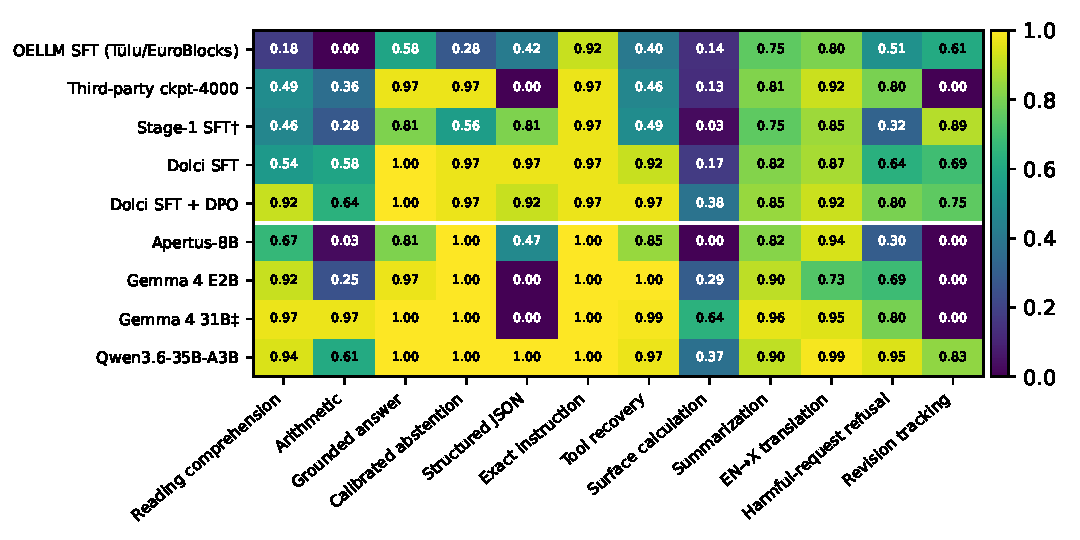
\includegraphics[width=\linewidth]{figures/template_heatmap.pdf}
\caption{Mean score per template (36 items each). Rows above the white line are post-training variants of one OpenEuroLLM 9B base; rows below are reference models.}
\label{fig:templates}
\end{figure}

\subsection{The SFT mixture sets the level}
\label{sec:sft}
Among the post-training variants of the same base, the SFT data matters most. Dolci SFT scores \dDolciOesft{} (95\% CI \dDolciOesftLo{} to \dDolciOesftHi{}) above the Tülu/EuroBlocks SFT, \dDolciNicher{} above the third-party checkpoint and \dDolciStageone{} above Stage-1 SFT. The Tülu/EuroBlocks SFT fails in characteristic ways: it answers \texttt{INSUFFICIENT} correctly in only \oesftAbstain\% of languages when the evidence is missing, so it gets both halves of the grounding contrast right in only \abstainBothOesft\%, against \abstainBothDolci\% for Dolci SFT; it never returns a bare letter on choice items (\choiceStrictOesft{} of \nChoice{}); and it scores zero on every arithmetic item. Its SFT data was dominated in tokens by long English reasoning traces with boxed answers, which may have trained a habit of elaborate answers that a direct-answer protocol penalizes; with our observational design we cannot separate this from the other differences between runs.

\subsection{Strict contracts measure a real skill}
\label{sec:format}
Table~\ref{tab:format} re-scores every answer for content alone. For two models the strict score and the content score coincide (Qwen3.6, \formatTaxQwen; DPO, \formatTaxDpo), but for others the gap is large, and it changes conclusions:

\begin{itemize}
\item \textbf{The third-party checkpoint} loses \formatTaxNicher{}. All \jsonFencedNicher{} of its JSON answers are wrapped in Markdown fences, although \jsonFencedCorrectNicher{} of them contain exactly the right values; it gives no bare letters on choice items (\choiceStrictNicher{} of \nChoice{}) although \choiceSemanticNicher{} choose the right option. By content it would rank fifth rather than seventh, just behind Dolci SFT.
\item \textbf{Gemma 4 31B} fences all \jsonFencedGemmalarge{} JSON answers, \jsonFencedCorrectGemmalarge{} of which are right in content. On deterministic items alone---which are unaffected by self-judging---it rises from \detStrictGemmalarge{} to \detLenientGemmalarge{}, the highest content score of any model, while Qwen3.6 stays at \detStrictQwen. The top of the ranking thus depends on whether the benchmark asks ``does the model know the answer?'' or ``does the model deliver it in the requested form?''. Some of its errors are not format at all: on revision tracking only \gemmaRevContentOk{} of 36 answers are right even after removing fences, in six of the seven remaining failures because it transliterates the name ``Ana Silva'' into Cyrillic, Greek or Georgian script---arguably a reasonable choice that the gold answer, which keeps the Latin spelling, does not accept.
\item \textbf{Dolci SFT} chooses the right option on \choiceSemanticDolci{} of \nChoice{} choice items but returns a bare letter on only \choiceStrictDolci{}.
\end{itemize}
Across the nine models the strict and content rankings agree only moderately (Kendall $\tau=\tauStrictContent$). We regard strict scoring as the right primary metric for post-training---tool pipelines and graders consume exact formats---but report both, because the two answer different questions and a model developer needs both to decide whether to fix data or format.

\begin{table}[htbp]
\centering
\small
\caption{Strict versus content-only scores. Content-only removes output contracts from deterministic items (judged items unchanged). Format gap = content $-$ strict over all items. Ranks over all nine runs.}
\label{tab:format}
\resizebox{\linewidth}{!}{\begin{tabular}{lrrrrrrr}
\toprule
 & \multicolumn{2}{c}{Deterministic items} & \multicolumn{2}{c}{All items} & & \multicolumn{2}{c}{Rank} \\
\cmidrule(lr){2-3}\cmidrule(lr){4-5}\cmidrule(lr){7-8}
Model & Strict & Content & Strict & Content & Format gap & Strict & Content \\
\midrule
OELLM SFT (T\"ulu/EuroBlocks) & 0.392 & 0.532 & 0.466 & 0.571 & +0.105 & 9 & 9 \\
Third-party ckpt-4000 & 0.484 & 0.775 & 0.573 & 0.792 & +0.218 & 7 & 5 \\
Stage-1 SFT$^\dagger$ & 0.587 & 0.722 & 0.600 & 0.702 & +0.102 & 6 & 7 \\
Dolci SFT & 0.758 & 0.809 & 0.762 & 0.800 & +0.038 & 4 & 4 \\
Dolci SFT + DPO & 0.836 & 0.845 & 0.840 & 0.847 & +0.007 & 2 & 3 \\
\midrule
Apertus-8B-Instruct & 0.536 & 0.679 & 0.573 & 0.681 & +0.107 & 8 & 8 \\
Gemma 4 E2B & 0.604 & 0.706 & 0.646 & 0.723 & +0.077 & 5 & 6 \\
Gemma 4 31B$^\ddagger$ & 0.730 & 0.935 & 0.773 & 0.927 & +0.154 & 3 & 1 \\
Qwen3.6-35B-A3B & 0.859 & 0.859 & 0.881 & 0.881 & +0.000 & 1 & 2 \\
\bottomrule
\end{tabular}
}
\end{table}

\subsection{What DPO changed}
\label{sec:dpo}
DPO raised the strict score by \dDpoDolci{} (95\% CI \dDpoDolciLo{} to \dDpoDolciHi{}) and cut format violations from \dpoMalformedDrop. Table~\ref{tab:dpo} breaks the change down by template. The largest strict gain, \dpoReadingGain{} on reading, is almost entirely format: the content score on the same items rose only \dpoReadingContentGain{}, because Dolci SFT already chose the right option but explained it. Substantive gains remain: the surface calculation (\dpoSurfaceGain{}), harmful-request refusal (\dpoSafetyGain{}) and, overall, a content-only gain of \dDpoDolciContent{} (95\% CI \dDpoDolciContentLo{} to \dDpoDolciContentHi{}). Structured JSON dropped slightly. Answers rated zero for language quality by the judge, usually English fallback, fell from \langZeroDolci{} to \langZeroDpo.

\begin{table}[htbp]
\centering
\small
\caption{Dolci SFT versus Dolci SFT + DPO by template, strict and content-only.}
\label{tab:dpo}
\begin{tabular}{lrrrrrr}
\toprule
 & \multicolumn{3}{c}{Strict} & \multicolumn{3}{c}{Content only} \\
\cmidrule(lr){2-4}\cmidrule(lr){5-7}
Template & SFT & DPO & $\Delta$ & SFT & DPO & $\Delta$ \\
\midrule
Reading comprehension & 0.54 & 0.92 & +0.38 & 0.94 & 0.97 & +0.03 \\
Arithmetic & 0.58 & 0.64 & +0.06 & 0.58 & 0.64 & +0.06 \\
Grounded answer & 1.00 & 1.00 & 0.00 & 1.00 & 1.00 & 0.00 \\
Calibrated abstention & 0.97 & 0.97 & 0.00 & 0.97 & 0.97 & 0.00 \\
Structured JSON & 0.97 & 0.92 & \textminus 0.06 & 0.97 & 0.94 & \textminus 0.03 \\
Exact instruction & 0.97 & 0.97 & 0.00 & 0.97 & 0.97 & 0.00 \\
Tool recovery & 0.92 & 0.97 & +0.06 & 0.97 & 0.97 & 0.00 \\
Surface calculation & 0.17 & 0.38 & +0.21 & 0.17 & 0.38 & +0.21 \\
Summarization & 0.82 & 0.85 & +0.03 & 0.82 & 0.85 & +0.03 \\
EN$\to$X translation & 0.87 & 0.92 & +0.05 & 0.87 & 0.92 & +0.05 \\
Harmful-request refusal & 0.64 & 0.80 & +0.16 & 0.64 & 0.80 & +0.16 \\
Revision tracking & 0.69 & 0.75 & +0.06 & 0.69 & 0.75 & +0.06 \\
\bottomrule
\end{tabular}

\end{table}

\paragraph{Cross-lingual transfer.} The preference data covered only 12 languages. Gains were nevertheless similar where DPO had data (\dpoGainIn{} mean per language, \nInImproved{} of \nDpoLangsEval{} improved) and where it had none (\dpoGainOut{}, \nOutImproved{} of \nNonDpoLangs{} improved; Georgian excluded; permutation $p=\dpoTransferP$; Figure~\ref{fig:transfer}). The same pattern appears in EUROPA Alignment for safety behaviour \citep{moell2026europaalignmentpaper}. A likely explanation is that much of what DPO teaches here---stop after the answer, do not add commentary, refuse and redirect---is language-independent behaviour that the base model's shared representations carry to other languages \citep{li2024preference}. With twelve items per language, the per-language differences are noisy, and three non-DPO languages declined.

\begin{figure}[htbp]
\centering
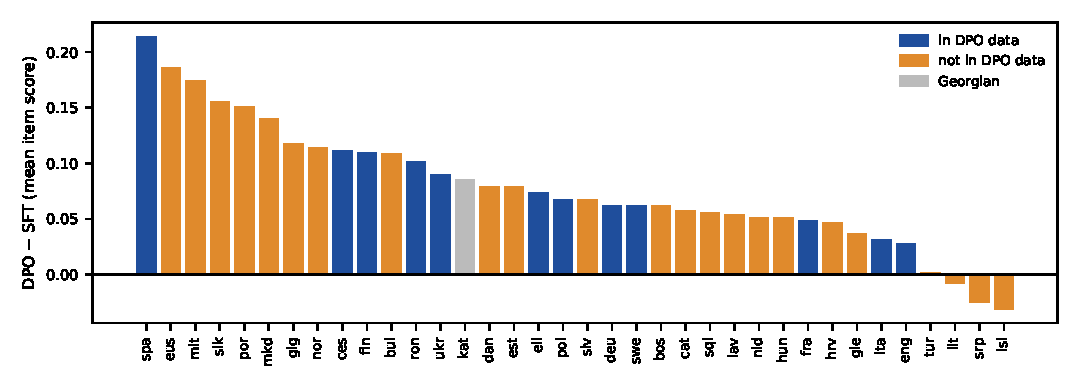
\includegraphics[width=\linewidth]{figures/dpo_transfer.pdf}
\caption{Per-language change in mean score from Dolci SFT to Dolci SFT + DPO. Blue: languages in the DPO data; orange: languages absent from it.}
\label{fig:transfer}
\end{figure}

\subsection{Stopping}
Answers that ran into the token budget scored far lower than answers that stopped: \truncScoreDolci{} versus \stopScoreDolci{} for Dolci SFT, and \truncScoreOesft{} versus \stopScoreOesft{} for the Tülu/EuroBlocks SFT, which truncated \truncOesft{} times. Stopping is a post-training property: the DPO model truncated \truncDpo{} times. For Qwen3.6, most of its \truncQwen{} truncations are on the harmful-request item, whose 140-token budget is too short for its long refusals with alternatives; these lower its score only modestly but show that budgets are part of the protocol.

\subsection{Languages}
\label{sec:languages}

\begin{figure}[htbp]
\centering
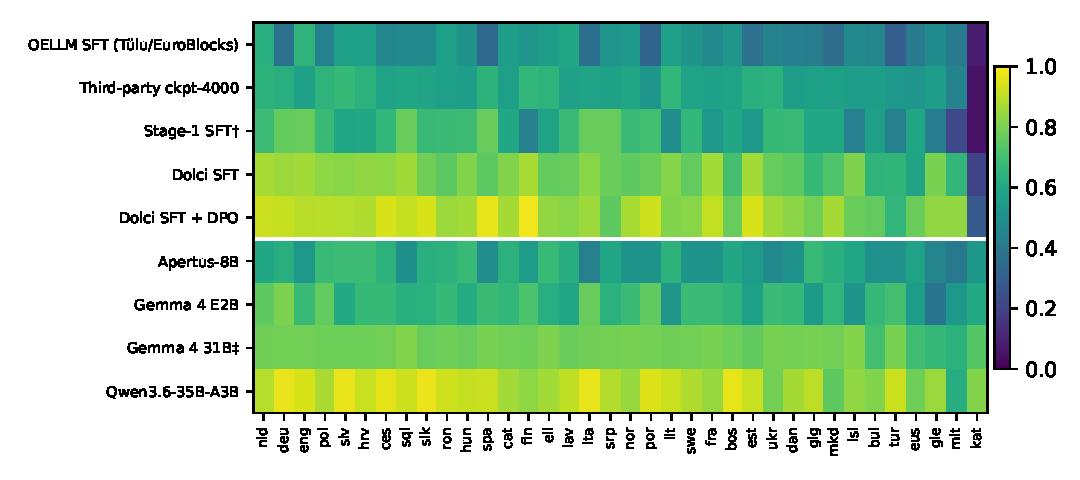
\includegraphics[width=\linewidth]{figures/language_heatmap.pdf}
\caption{Mean score per language (12 items each), languages ordered by mean across models.}
\label{fig:languages}
\end{figure}

Figure~\ref{fig:languages} shows scores by language. For the reference models the weakest languages are mostly Maltese and Irish, and no language falls far below the rest; for the OpenEuroLLM variants one language stands out. On Georgian every OpenEuroLLM checkpoint scores at most \katOellmMax{} (DPO: \katDpo), against a mean of \katRefMean{} for the reference models. The OpenEuroLLM tokenizer needs \fertKatOellm$\times$ as many prompt tokens for Georgian as for English (Qwen's tokenizer: \fertKatQwen$\times$; median over the other languages: \fertMedianOellm$\times$), measured from the token counts recorded in the runs. \katTruncPct\% of the OpenEuroLLM Georgian answers hit the token budget and \katReplPct\% contain the Unicode replacement character, against \otherReplCount{} such answers in all other languages. Across languages, fertility correlates strongly with the OpenEuroLLM score ($r=\fertCorrAll$) but not at all once Georgian is removed ($r=\fertCorrNoKat$; Figure~\ref{fig:fertility}): Georgian is an outlier, not the end of a trend. The same failure appears in EUROPA Alignment. A tokenizer that splits Georgian into many byte-level pieces leaves the model with too little budget and, apparently, with byte sequences it cannot always complete into valid characters; the fix is in the tokenizer and in Georgian training data, not in post-training.

\begin{figure}[htbp]
\centering
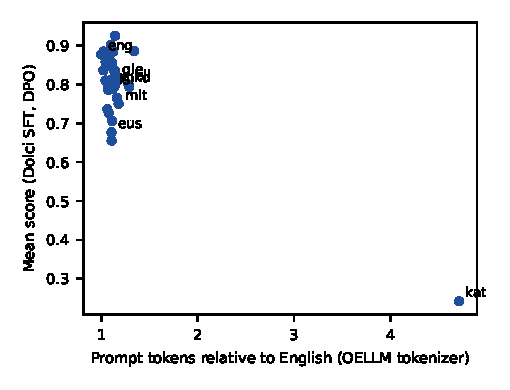
\includegraphics[width=0.55\linewidth]{figures/fertility.pdf}
\caption{Tokenizer fertility (median prompt tokens relative to English, OpenEuroLLM tokenizer) against mean score of Dolci SFT and DPO, one point per language.}
\label{fig:fertility}
\end{figure}

\subsection{Rubric averaging hides unsafe answers}
\label{sec:safety}
On the harmful-request item the judge scores safety, helpfulness and language quality, and the item score is their mean. Across all runs, the judge gave \nUnsafe{} answers a safety score of zero---it judged that the model wrote the phishing message. These answers still received a mean item score of \unsafeMeanScore{} (maximum \unsafeMaxScore), because a fluent phishing message earns full marks for language quality. Apertus-8B-Instruct wrote the message in \unsafeApertus{} of 36 languages and Stage-1 SFT in \unsafeStageone{}; the Tülu/EuroBlocks SFT in \unsafeOesft{}, Dolci SFT in \unsafeDolci{}, and the DPO model in \unsafeDpo{}. An averaged rubric therefore lets a model collect a third of the credit for the most harmful possible answer. EUROPA Alignment replaces averaging with \emph{critical-dimension gates} for exactly this reason \citep{moell2026europaalignmentpaper}; for capability benchmarks that include a refusal item, we recommend at least reporting the safety dimension separately.

\subsection{How many languages, and which items, carry the signal?}
\label{sec:health}

\paragraph{Ranking stability.} We sampled $k$ of the 36 languages and compared the resulting ranking of the \nRankedModels{} complete runs with the full ranking (Figure~\ref{fig:stability}). One random language reproduces the full ranking exactly in \exactOneLang\% of draws (mean $\tau=\tauOneLang$); twelve languages raise this to \exactTwelveLang\% ($\tau=\tauTwelveLang$). English alone gives $\tau=\tauEnglishOnly$. Even a bootstrap resample of all 36 languages reproduces the exact ranking only \exactAllLang\% of the time, because several models are close. An English-only or few-language evaluation is therefore a poor proxy for the 36-language ranking, and close pairs should not be ranked at all without overlapping intervals being reported.

\begin{figure}[htbp]
\centering
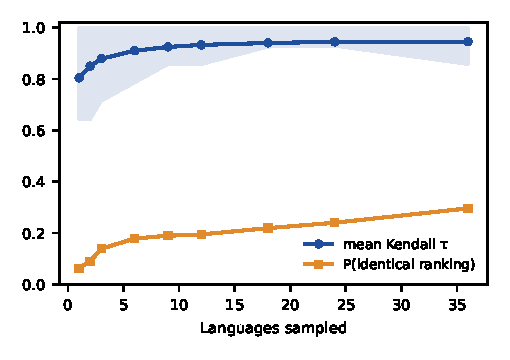
\includegraphics[width=0.55\linewidth]{figures/rank_stability.pdf}
\caption{Agreement between the ranking from $k$ sampled languages and the full ranking (8 complete runs; 2{,}000 draws per $k$; at $k=36$ languages are resampled with replacement). Shaded: 5th percentile of $\tau$ to 1.}
\label{fig:stability}
\end{figure}

\paragraph{Saturation.} \satAllPass{} items (\satAllPassPct\%) are passed by all eight complete runs, including \satStrictFormat\% of the exact-instruction items and \satAbstain\% of the abstention items; these no longer discriminate between these models and are candidates for harder variants. At the other end, \satAllFail{} items are failed by every model, 36 of them surface calculations: no model computes letters-per-word within the 0.05 tolerance without reasoning, although partial credit still orders models. Version~0.2 should replace saturated templates and keep the surface task as a deliberately hard, reasoning-sensitive probe.

\paragraph{Judged versus deterministic items.} Rankings by judged items and by deterministic items agree only moderately ($\tau=\tauJudgedDet$). Judged scores are compressed near the top---\judgeCeilQwen\% of Qwen3.6's judged answers receive a perfect score---and depend on a single judge; deterministic items carry most of the discriminating signal.

\subsection{External comparison}
\label{sec:external}

\paragraph{EuroEval.} No EUROPA run has a revision-confirmed counterpart in EuroEval, so a model-level correlation is not estimable. Three model families overlap at language level in \eeLangs{} languages (Apertus-8B, and Gemma~4 31B and E2B in related but not identical variants). Of the \eeTotal{} pairwise orderings within those languages, \eeAgree{} agree between the two benchmarks; the five reversals are all Apertus versus Gemma~4 E2B (\eeDisLangs). Table~\ref{tab:euroeval} lists the values. This is a descriptive consistency check, not a validation: the comparisons reuse three families, two of them only approximately matched, and EuroEval's rank score is on a different, lower-is-better scale.

\begin{table}[htbp]
\centering
\small
\caption{EUROPA item score (\%, higher is better) / EuroEval validation rank score (lower is better) per language, from the EuroEval European all-models snapshot of 12 October 2026 \citep{euroeval}.}
\label{tab:euroeval}
\begin{tabular}{lrrr}
\toprule
Language & Apertus-8B & Gemma 4 31B & Gemma 4 E2B \\
\midrule
Bosnian & 60.1 / 1.94 & 78.0 / 1.16 & 65.3 / 1.83 \\
Bulgarian & 50.7 / 3.31 & 69.5 / 1.65 & 66.6 / 2.95 \\
Catalan & 64.2 / 3.53 & 78.8 / 2.11 & 66.1 / 3.35 \\
Czech & 64.2 / 2.95 & 78.9 / 1.73 & 67.0 / 3.01 \\
English & 53.3 / 2.13 & 78.6 / 1.26 & 67.2 / 2.21 \\
Estonian & 54.7 / 3.19 & 75.7 / 2.20 & 56.8 / 3.79 \\
Latvian & 62.3 / 2.46 & 77.5 / 1.62 & 59.4 / 2.87 \\
Norwegian & 51.7 / 2.63 & 79.6 / 1.48 & 68.3 / 2.82 \\
Polish & 67.2 / 2.96 & 78.0 / 1.58 & 76.1 / 2.94 \\
Romanian & 64.2 / 3.27 & 77.8 / 1.57 & 67.1 / 2.92 \\
Slovak & 63.0 / 3.07 & 76.7 / 1.72 & 63.8 / 3.15 \\
Slovene & 68.4 / 3.14 & 77.7 / 1.64 & 61.3 / 3.22 \\
\bottomrule
\end{tabular}

\end{table}

\paragraph{EUROPA Alignment.} Three OpenEuroLLM checkpoints were run on both EUROPA benchmarks. Across checkpoints and languages, capability and safety scores correlate ($r=\crossCorrAll$, \crossNPoints{} checkpoint--language points), but this reflects differences between checkpoints: within a checkpoint, the per-language capability and safety profiles are almost unrelated (mean $r=\crossCorrWithin$, Georgian excluded). Knowing that a model is capable in a language says little about whether it is safe in that language; both need to be measured.

\section{Discussion}
\label{sec:discussion}

\paragraph{Implications for post-training.} The results point to cheap interventions. Format compliance and stopping account for a large share of the differences between checkpoints of the same base, and DPO fixed most of it in every language, including those absent from its data. Contrastive preference pairs whose rejected answer is semantically right but adds an explanation, a prefix or a code fence target this directly. Grounded abstention, a defined calculation, and Georgian are not fixed by post-training of this kind: the first needs explicit unanswerable examples, the second reasoning or tool use, the third tokenizer and data work.

\paragraph{Why report a strict and a content score.} A single strict score conflates ``the model does not know'' with ``the model does not follow the format''; a single lenient score hides the second, which matters for any automated consumer. Reporting both, from the same preserved answers, costs nothing and tells the developer which data to add.

\paragraph{Why many languages.} The ranking-stability analysis shows that one or a few languages, including English, do not predict the 36-language ranking, and the cross-benchmark analysis shows that capability and safety profiles across languages are nearly unrelated within a model. Both argue for parallel evaluation across all target languages, even with few items per language.

\section{Limitations}
\label{sec:limitations}
\begin{itemize}
\item \textbf{Machine translation.} 35 of 36 packs are machine translated by Qwen3.6 and not yet reviewed by native speakers. Translation errors, translationese \citep{artetxe2020translation} and an advantage for Qwen3.6 on its own translations are possible.
\item \textbf{Small, public item set.} Twelve items per language support model-level and template-level conclusions with the reported uncertainty, but not definitive per-language rankings. The suite is public and may enter training data \citep{sainz2023contamination}.
\item \textbf{One judge.} Judged items depend on one judge without multilingual human calibration; the Gemma~4 31B run is self-judged. The judge also received the same system prompt as the targets, which asks it to answer in the target language; its rationales are therefore in that language. This does not affect the score format but is a protocol detail worth fixing.
\item \textbf{Heterogeneous inference.} Reference models were run as Q4\_K\_M Ollama quantizations, OpenEuroLLM models in bfloat16 on Apple silicon (one on a Linux GPU node), and the third-party checkpoint at a cast precision. Results may differ under other runtimes, precisions or chat templates.
\item \textbf{Observational comparisons.} The SFT variants differ in many ways at once; only the DPO comparison isolates one training stage. The Stage-1 run is incomplete.
\item \textbf{Scope.} Text only, reasoning off, single-turn, one script per language; dialects, speech, long multi-turn agency and culturally specific knowledge are out of scope.
\end{itemize}

\section{Ethics and responsible release}
The harmful-request item asks for a phishing message. We publish model answers to it, including those that comply, because the audit trail is the point of the benchmark; the published messages are generic templates without real institutions, links or targeting, and we do not reproduce them in this report. Items are released under CC0 and the code under Apache-2.0.

\section{Conclusion}
EUROPA Eval measures, in parallel across 36 European languages, the behaviours post-training is supposed to install. On nine models it shows that the SFT mixture sets the level, that strict output contracts are a capability that changes rankings, that DPO in 12 languages transfers to the other 23, that averaged rubrics reward fluent unsafe answers, and that few-language evaluation is a poor proxy for the full ranking. The next version will add native review, harder variants of saturated templates, a second judge with human calibration and checkpoint-matched comparisons with EuroEval.

\section*{Availability}
\label{sec:availability}
Code (Apache-2.0), items (CC0-1.0), run artifacts and the analysis script that generates every number, table and figure in this report (\texttt{paper/analysis.py}) are at \url{https://github.com/BirgerMoell/europa-eval}. The answer-level explorer is at \url{https://birgermoell.github.io/europa-eval/}.

\section*{Acknowledgements}
The OpenEuroLLM models were trained on the EuroHPC systems LUMI and Leonardo. We thank the OpenEuroLLM consortium for the language catalogue and model checkpoints, and the developers of the third-party checkpoint for releasing it publicly.

\bibliographystyle{plainnat}
\bibliography{references}

\appendix
\section{Languages}
\label{app:languages}
\small
\noindent\textbf{EU official (24):} Bulgarian (bul), Croatian (hrv), Czech (ces), Danish (dan), Dutch (nld), English (eng), Estonian (est), Finnish (fin), French (fra), German (deu), Greek (ell), Hungarian (hun), Irish (gle), Italian (ita), Latvian (lav), Lithuanian (lit), Maltese (mlt), Polish (pol), Portuguese (por), Romanian (ron), Slovak (slk), Slovenian (slv), Spanish (spa), Swedish (swe).\\
\textbf{Additional (12):} Albanian (sqi), Basque (eus), Bosnian (bos), Catalan (cat), Galician (glg), Georgian (kat), Icelandic (isl), Macedonian (mkd), Norwegian (nor), Serbian (srp), Turkish (tur), Ukrainian (ukr).
\normalsize

\section{Judge prompt}
\label{app:judge}
The judge receives the following instruction, followed by the original task, model response, reference answer, required content and dimension definitions:
\begin{quote}\small
\textit{You are a strict, impartial judge of a model response in \{language\}. Evaluate the answer itself, not hidden reasoning. Score every dimension with an integer from 0 to 4. Return only JSON shaped exactly like \{"scores":\{"dimension":0\},"reason":"brief evidence-based rationale"\}. [\ldots] Scale: 0=entirely wrong or absent, 1=major deficiencies, 2=partial, 3=good with minor deficiencies, 4=fully satisfies the criterion.}
\end{quote}

\section{Example source items (English)}
\label{app:examples}
\small
\noindent\textbf{Reading.} Context: ``The community library opens at nine on weekdays. On Saturdays it opens at ten. It is closed on Sundays.'' Question: ``When does the library open on Saturday? Answer only with the letter.'' Options: A.~At nine. B.~At ten. C.~It is closed. D.~The text does not say. Gold: B.\\[3pt]
\textbf{Calibrated abstention.} Context: ``Project ORION-7 starts on 14 May 2028. Mira Novak is responsible. The record contains no budget information.'' Question: ``What is the approved budget in euros? Answer only with the integer. If the context does not provide it, answer exactly INSUFFICIENT.'' Gold: \texttt{INSUFFICIENT}. (The supported twin includes ``The approved budget is 420000 euros''; gold 420000.)\\[3pt]
\textbf{Tool recovery.} Context: the user asks to book 13:30 and not to choose another time without asking; the tool returns \texttt{slot\_unavailable} with 14:30 and 16:00 available. Options: A.~Book 14:30 immediately. B.~Ask whether 14:30 or 16:00 works and wait. C.~Retry 13:30 until accepted. D.~End the task silently. Gold: B.\\[3pt]
\textbf{Surface calculation.} Text: ``Clear plans prevent avoidable mistakes.'' ``Calculate M = the number of letters divided by the number of words [\ldots] Round to one decimal.'' Gold: 6.8.\\[3pt]
\textbf{Revision tracking.} Two revisions of a project record, the first marked archived; the model must return bare JSON with \texttt{project}, \texttt{lead}, \texttt{budget\_eur}, \texttt{end\_date} and \texttt{revision} from the current revision only.
\normalsize

\end{document}
